\documentclass[11pt,a4paper]{report} 
% Für doppelseitigen Ausdruck (nur bei > 60 Seiten sinnvoll)
% \usepackage{ifthen}
% \setboolean{@twoside}{true}
% \setboolean{@openright}{true} 

% Deutsch
\usepackage[german]{babel} % deutsch und deutsche Rechtschreibung
\usepackage[utf8]{inputenc} % Unicode Text 
\usepackage[T1]{fontenc} % Umlaute und deutsches Trennen
\usepackage{textcomp} % Euro
\usepackage[hyphens]{url}
% statt immer Ab\-schluss\-ar\-beit zu schreiben
% einfach hier sammeln mit -. 
\hyphenation{Ab-schluss-ar-beit}
% Vorsicht bei Umlauten und Bindestrichen
\hyphenation{Ver-st\"ar-ker-aus-gang}
 % eigene Hyphenations, die für das Dokument gelten
\usepackage{amssymb} % Symbole
\usepackage{emptypage} % Wirklich leer bei leeren Seiten

%% Fonts, je ein kompletter Satz an Optionen

% Times New Roman, gewohnter Font, ok tt und serifenlos
%\usepackage{mathptmx} 
%\usepackage[scaled=.95]{helvet}
%\usepackage{courier}

% Palatino mit guten Fonts für tt und serifenlos
\usepackage{mathpazo} % Palatino, mal was anderes
\usepackage[scaled=.95]{helvet}
\usepackage{courier}

% New Century Schoolbook sieht auch nett aus (macht auch tt und serifenlos)
%\usepackage{newcent}

% Oder default serifenlos mit Helvetica 
% ich kann es nicht mehr sehen ...
%\renewcommand{\familydefault}{\sfdefault}

% ein bisschen eine bessere Verteilung der Buchstaben...
\usepackage{microtype}

% Bilder und Listings
\usepackage{graphicx} % wir wollen Bilder einfügen
\usepackage{subfig} % Teilbilder
\usepackage{wrapfig} % vielleicht doch besser vermeiden
\usepackage{listings} % schöne Quellcode-Listings
% ein paar Einstellungen für akzeptable Listings
\lstset{basicstyle=\ttfamily, columns=[l]flexible, mathescape=true, showstringspaces=false, numbers=left, numberstyle=\tiny}
\lstset{language=python} % und nur schöne Programmiersprachen ;-)
% und eine eigene Umgebung für Listings
\usepackage{float}
\newfloat{listing}{htbp}{scl}[chapter]
\floatname{listing}{Listing}

% Seitenlayout
\usepackage[paper=a4paper,width=14.8cm,left=30mm,right=30mm,height=23cm]{geometry}
\usepackage{setspace}
\linespread{1.15}
\setlength{\parskip}{0.5em}
\setlength{\parindent}{0em} % im Deutschen Einrückung nicht üblich, leider

% Seitenmarkierungen 
\newcommand{\phv}{\fontfamily{phv}\fontseries{m}\fontsize{9}{11}\selectfont}
\usepackage{fancyhdr} % Schickere Header und Footer
\pagestyle{fancy}
\renewcommand{\chaptermark}[1]{\markboth{#1}{}}
%\fancyhead[L]{\phv \leftmark}
\fancyhead[RE,LO]{\phv \nouppercase{\leftmark}}
\fancyhead[LE,RO]{\phv \thepage}
% Unten besser auf alles Verzichten
%\fancyfoot[L]{\textsf{\small \kurztitel}}
\fancyfoot[C]{\ } % keine Seitenzahl unten
%\fancyfoot[R]{\textsf{\small Technische Informatik}}

% Theorem-Umgebungen
\newtheorem{definition}{Definition}[chapter]
\newtheorem{satz}{Satz}[chapter]
\newtheorem{lemma}[satz]{Lemma} % gleicher Zähler wie Satz
\newtheorem{theorem}{Theorem}[chapter]
\newenvironment{beweis}[1][Beweis]{\begin{trivlist}
\item[\hskip \labelsep {\textit{#1 }}]}{\end{trivlist}}
\newcommand{\qed}{\hfill \ensuremath{\square}}

%% Quellen
% Eine Alternative wäre Quellen in Literatur und Online-Quellen
% zu teilen
% \usepackage{bibtopic} 

% Hochschule Logo, noch nicht perfekt
\usepackage{hsmalogo}

% Spezialpakete
\usepackage{epigraph}
\setlength{\epigraphrule}{0pt} % kein Trennstrich

% damit wir nicht so viel tippen müssen, nur für Demo 
\usepackage{blindtext} 

% ifthen für sperrvermerk
\newif\ifsperrvermerk
 % alle Pakete und Einstellungen

% Hier anpassen 
\newcommand{\autor}{Nicolas Pawelka}
\newcommand{\matrikelnummer}{2120666}
\newcommand{\fachsemester}{5} % im wie vielten Semester waren Sie?
\newcommand{\studiengang}{Medizintechnik}
%\newcommand{\studiengang}{Technische Informatik}
%\newcommand{\studiengang}{Informationstechnik}
\newcommand{\firma}{NewTec GmbH}
\newcommand{\standort}{Mannheim}
\newcommand{\abteilung}{Embedded Software}
\newcommand{\betreuer}{Julia Kammerer}
\newcommand{\pbeginn}{4.9.2023}
\newcommand{\pende}{29.2.2024}
\newcommand{\tage}{111} % arbeitstagerechner verwenden!
\newcommand{\titel}{Bericht zum praktischen Studiensemester}
\newcommand{\kurztitel}{Praxisbericht}
\sperrvermerktrue % Kommentar am Anfang der Zeile löschen für Sperrvermerk

% Wenn jemand unbedingt ein Glossar will, die nächsten drei Zeilen...
%\usepackage{glossaries} % oder schlimmer mit [toc], damit es im TOC auftaucht
%\makeglossaries
%\newglossaryentry{Computer}{name=Computer,
  description={Eine programmierbare Maschine, die Eingaben erhält, Daten speichert und manipuliert
    und Ausgaben in einem sinnvollem Format ausgibt. (Und wer so was in ein Glossar eines Berichts
    für einen technischen Studiengang schreibt hat es nicht verstanden)}}
\newglossaryentry{naiv}{name=na\"{\i}ve,
  description={Ein franzöisches Lehnswort (Adjektiv, Form von naïf)
    Erweckt den Eindruch oder hat mangelnde Erfahrung, mangelndes Verständnis oder mangelnde Skills}}
\newglossaryentry{Linux}{name=Linux,
  description={Generischer Ausdruck für eine Familie von Unix-artigen Betriebssystemen die den
    Linux-Kernel verwenden},
  plural=Linuces}
\newacronym[longplural={Frames per Second}]{fpsLabel}{FPS}{Frame per Second}
\newacronym{acme}{ACME}{A Company Making Everything}
\newglossaryentry{Praktisches Studiensemester}{name=Praktisches Studiensemester,
  description={Im Rahmen des Ingenieursstudiums ein Semester in der betrieblichen Praxis
    zur Ergänzung und Vertiefung des Studienwissens durch selbstständige ingenieurnahe Tätigkeit
    betreut durch einen Ingenieur des Betriebes}}
 % In dieser Datei die Einträge definieren
% und noch ganz unten printglossaries auskommentieren
% Damit jetzt ein Glossar gezeigt wird noch \gls{label} verwenden

\begin{document}
\begin{titlepage}
  \hsmalogo[1] \hfill
  \parbox[b]{60mm}{
    Fakultät Informationstechnik\\
    Studiengang \studiengang}
  \begin{center}
    \rule{1\textwidth}{1pt}\\[-3mm]
    \parbox[t][64mm]{110mm}{% 11 cm für Breite 13, ca. 7 für Höhe 6
      \Large{\ } \\[8mm]
      Bericht zum praktischen Studiensemester \\[4mm]
      \begin{tabular}{rl}
        \large{Vorgelegt von} & \large{\autor} \\[2mm]
        \large{Studiengang} & \large{\studiengang} \\[2mm]
        \large{Firma} & \large{\firma} \\[2mm]
      \end{tabular}
    }
    \rule{\textwidth}{1pt}    
    \vfill    
  \end{center}

  \vspace{2em}
  \begin{tabular}{ll}
    Name & \autor \\
    Matrikelnummer & \matrikelnummer \\
    Studiengang & \studiengang \\
    Fachsemester & \fachsemester \\[8mm]

    Praktikumszeitraum & \pbeginn\ \ bis \ \pende \\
    Präsenztage & \tage \\[8mm]
    
    Firma & \firma \\
    Standort & \standort \\
    Abteilung & \abteilung \\
    Betreuer & \betreuer \\
  \end{tabular}
  
  \vspace{8em}
  \noindent\begin{tabular}{p{0.48\textwidth}p{0.48\textwidth}}
             \rule{0.46\textwidth}{0.5pt} & \rule{0.46\textwidth}{0.5pt}  \\
             Datum, \betreuer & Firmenstempel
           \end{tabular}
  \vfill
\end{titlepage}
\cleardoublepage


% Erklärung gemäß der Prüfungsordnung
\thispagestyle{empty}
\subsection*{Selbstständigkeitserklärung}

Ich versichere, dass ich diesen Bericht zum praktischen Studiensemester
selbstständig und nur unter Verwendung der angegebenen Quellen und
Hilfsmittel angefertigt habe.
Die Stellen, an denen Inhalte aus den Quellen verwendet wurden, sind
als solche eindeutig gekennzeichnet.
Die Arbeit hat in gleicher oder ähnlicher Form bei keinem anderen
Prüfungsverfahren vorgelegen.

\vspace{6em}
\noindent\begin{tabular}{p{0.48\textwidth}p{0.48\textwidth}}
\rule{0.42\textwidth}{0.5pt} & \rule{0.48\textwidth}{0.5pt}\\
Datum, Ort                   & \makebox[1cm]{\ } \autor
\end{tabular}

\vfill

\ifsperrvermerk
\subsection*{Sperrvermerk}

Der vorliegende Bericht enthält interne und teilweise vertrauliche Daten
der Firma \newline \firma.
Der Bericht darf daher zu keinen anderen als Prüfungszwecken verwendet werden.
Insbesondere ist die Vervielfältigung und Veröffentlichung von Berichtinhalten
oder Teilen davon nur mit Zustimmung des Unternehmens erlaubt.
\vfill
\fi

\cleardoublepage

 % Titelseite, Erklärungen, etc.

\begin{abstract}
Während des praktischen Studiensemesters bei der \firma wurden verschiedene Projekte behandelt, die einen umfassenden Einblick in die Welt der Softwareentwicklung geben konnten.

Zunächst wird mittels des Tools \glqq Doxygen\grqq{} aber auch den Programmiersprachen HTML, CSS und JavsScript eine moderne und benutzerfreundliche Vorlage zur Dokumentaion von Quellcode gestaltet. Neben graphischem Design werden auch dynamische Elemente wie Button implementiert.

Im zweiten Projekt wird als Teil einer Bachelorarbeit eine Schnittstelle zwischen den Office Tools MS Project und MS Excel entwickelt. Diese basiert auf den Programmiersprachen VBA und Python und soll die Vorteile beider vereinen.

Abschließend wird geprüft ob die Entwicklung und Anpassung eines lokalen Language Models (LLM) für die Generierung von Code-Dokumentation mit momentan vorhandenen Ressourcen umsetzbar ist.

Neben den aufgeführten Projekten wurde noch weitere Aufgaben durchgeführt, die auf Grund ihres geringen Umfangs keine Beachtung in diesem Bericht finden.

\end{abstract}

\tableofcontents

\chapter{Vorstellung des Unternehmens und der Abteilung} \label{chap:einf}
\section{Das Unternehmen} \label{sec::company}

Die NewTec GmbH ist ein mittelständisches Unternehmen mit Sitzen in Mannheim, Pfaffenhofen, Bremen, Freiburg und Markdorf. Gegründet im Jahr 1986 hat sich NewTec zu einem führenden Anbieter in den Bereichen Embedded Systems, Softwareentwicklung und Systemintegration. Das Unternehmen bietet Dienstleistungen für Kunden aus verschiedenen Branchen wie der Automobilindustrie, Medizintechnik, Luft- und Raumfahrt sowie Industrieautomation an. Es legt großen Wert auf eine enge Zusammenarbeit mit seinen Kunden, um deren individuelle Anforderungen bestmöglichst zu erfüllen. Einen großen Teil des Portfolios besteht aus der Entwicklung von sicheren Systemen, wobei dieser Bereich in funktionale Sicherheit und embedded Security unterteilt werden kann.


\section{Die Abteilung}

Im Standort Mannheim sind drei Teams tätig, die sich auf Hardwareentwicklung, Softwareentwicklung und Funktionale Sicherheit spezialisiert haben. Das Praxissemester wird im Bereich der Softwareentwicklung durchgeführt.

\chapter{Entwicklung eines Doxygen-Templates zur Schaffung einer
zeitgemäßen und übersichtlichen Codebasis} \label{chap:ppv}

In der Welt der Softwareentwicklung ist es wie in einem gut geführten Buch, der Code sollte
klar und leicht verständlich sein. Jedoch reicht in den meisten Fällen der rohe Quellcode nicht
zum Verständnis aus. Durch gezielte Kommentare sollten Entwickler ihr Programm zur besseren Wartung
dokumentieren. Dieses Kapitel befasst sich mit der Entwicklung eines 
Doxygen -Templates, das die Dokumentation nicht nur funktional, sondern auch zeitgemäß und
benutzerfreundlich gestaltet. Das Ziel ist es, den Entwicklern ein Werkzeug an die Hand zu 
geben, mit dem sie nicht nur effizient dokumentieren können, sondern auch einen klaren Blick auf
die Struktur ihres Codes behalten.

\section{Analyse der bestehenden Code-Dokumentation} \label{sec:was}

\subsection{Allgemeines}
Im Softwareengineering gibt es verschiedene Arten der Dokumentation. Hierbei wären zu nennen die 
Benutzerdokumentation, Installationsdokumentation, Datendokumentation, Testdokumentation oder die 
Entwicklungsdokumentation etc.\cite{Beningo} Beispielsweise dient die Benutzerdokumentation meist als Anleitung für den Endnutzer, bei der Installationsdokumentation werden Vorbedingungen an der Hardware- oder Softwareumgebung definiert oder die Entwicklungsdokumentation hält die Stakeholder Anforderungen in Form einens Lasten- und Pflichtenheft fest \cite{Lehner}.

\newpage
\newgeometry{bottom=1mm}
\noindent
Wenn eine Dokumentation zur Beschreibung des Quellcodes dient, bezeichnet man diese als Programmiererdokumentation. Diese Art der Dokumentation zu schreiben und stets auf dem aktuellsten Stand zu halten ist für jedes Softwareprojekt sehr wichtig und wertvoll. Eine gut geschriebene Dokumentation reduziert nicht nur die Einarbeitungszeit neuer Teammitglieder erheblich, sondern minimiert auch den allgemeinen Wartungsaufwand. Dadurch wird vermieden, dass für eine kleine Änderung zunächst eine umfangreiche Codebasis durchsucht und debuggt werden muss \cite{Beningo}. Dies führt zu erheblichen Einsparungen, sowohl in finanzieller Sicht als auch vor allem in Bezug auf den zeitlichen Aufwand \cite{Lehner}. In den Anfängen der Programmierung war es üblich, diese Dokumentation klein gegliedert auf einem eigenen Dokument aufzuführen \cite{Lehner}. Die Schnelligkeit und das Volumen mit der heutzutage Änderungen an Quellcode vorgenommen werden kann, lässt dieses Verfahren nicht mehr zu.

\noindent
In der modernen Softwaredokumentation wird eine andere Herangehensweise verfolgt. Hierbei sind zwei Aspekte für dieses Projekt hervorzuheben: Einerseits sollte die Dokumentation idealerweise direkt in den Code integriert werden. Andererseits wird die Verwendung von Dokumentationswerkzeugen wie bspw. Javadoc oder Doxygen empfohlen, um eine unterstützende Ansicht zu ermöglichen \cite{Lehner}. Im Rahmen dieser Arbeit wird nicht näher auf Javadoc eingegangen, sondern Doxygen detailiertet beleuchtet. 

\subsection{Doxygen} \label{sub:Doxygen}

Doxygen gilt als eines der führenden Software-Dokumentationswerkzeuge, insbesondere für die Programmiersprachen C und C++ \cite{Beningo}. Es ermöglicht einem, verschieden Arten von Daten wie beispielsweise Bilder, Tabellen oder Gleichungen in die jeweilige Dokumentation einzuschließen. Da es sich um ein Open Source Projekt handelt, kann der komplette Quellcode auf GitHub, einer Plattform für die Versionskontrolle von Softwareprojekten, eingesehen und bei Bedarf angepasst werden \cite{doxygen_git}.

\noindent
Bei der Analyse des geschriebenen Codes, sucht Doxygen nach einem spezifischen Zeichensatz, der darauf hinweist, dass der entsprechende Kommentar für Doxygen geschrieben wurde. Hierbei werden Kommentarblöcke im Stile der Sprache C verfasst. Einziger Unterschied ist, dass ein zweites \glqq  *  \grqq{}- Symbol zu Beginn des Kommentars hinzugefügt wird \cite{Beningo}. Doxygen generiert dann aus diesen Kommentaren z.B. eine HTML- Ausgabe. Diese kann dann durch das Aufrufen der \glqq index.hmtl \grqq{}- Datei angezeigt werden.

\noindent
Ein weiterer Vorteil der von Doxygen generierten Dokumentation ist die Einbindung von LaTeX, wodurch direkt eine komplette PDF-Datei erzeugt werden kann. Neben den beiden genannten Ausgaben unterstützt Doxygen noch weiter Typen, wie z.B  CHM, XML,  RTF,  PostScript,  Manpages oder Markdown \cite{doxygen}.
 \begin{figure}[H]
    \centering
    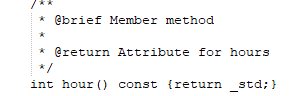
\includegraphics{images/Doxygen_Example.png}
    \caption{Dokumentation einer Methode}
    \label{fig:doxygen-example}
\end{figure}



\section{Anforderungsdefinitionen für das Template} \label{sec:Requirments}

Momentan wird die von Doxygen standardmäßig erzeugte Dokumentation genutzt (siehe \ref{fig:doxygen-befor}). Diese weist eine veraltete visuelle Gestaltung auf, die nicht mehr zeitgemäß ist. Eine modernere Optik trägt zu einer ansprechenderen und leichter zugänglichen Präsentation der Software bei, wodurch die Benutzerfreundlichkeit sowie die Lesbarkeit verbessert wird. Auf dieser Vorlage basierend sollen die folgenden Anforderungen erfüllt werden:
\begin{enumerate}[label=\textbf{A.\arabic*}]
    \item \label{req:Layout} Modernes Layout mit NewTec-Branding
    \item \label{req:Notes} Möglichkeit zur Einbindung von farblich hervorgehobenen Paragraphen, wie beispielsweise Notes bzw. Hinweise, Warnungen, Probleme im Code oder veralteter Funktionen.
    \item \label{req:Darkmode} Implementierung eines Dunkelmodus, inklusive eines Buttons, um zwischen Hell- und Dunkelmodus wechseln zu können.
    \item \label{req:Copy} Wenn Codeabschnitte in die Dokumentation integriert werde, die Möglichkeit bieten diesen Abschnitt per Copy-to-Clipboard Button zu übernehmen, sowie eine direkte Möglichkeit diesen Code zu editieren.
    \item \label{req:Search} Suchleiste mit detaillierterer Filterung nach Methoden, Klassen und Funktionen.
    \item \label{req:PDF} PDF-Generierung mit LaTeX per Button auf der Website. Dies ermöglicht eine Erstellung direkt innerhalb der Dokumentation, ohne zusätzliche Schritte über die Kommandozeile zu gehen.
\end{enumerate}


\begin{figure}[H]
    \centering
     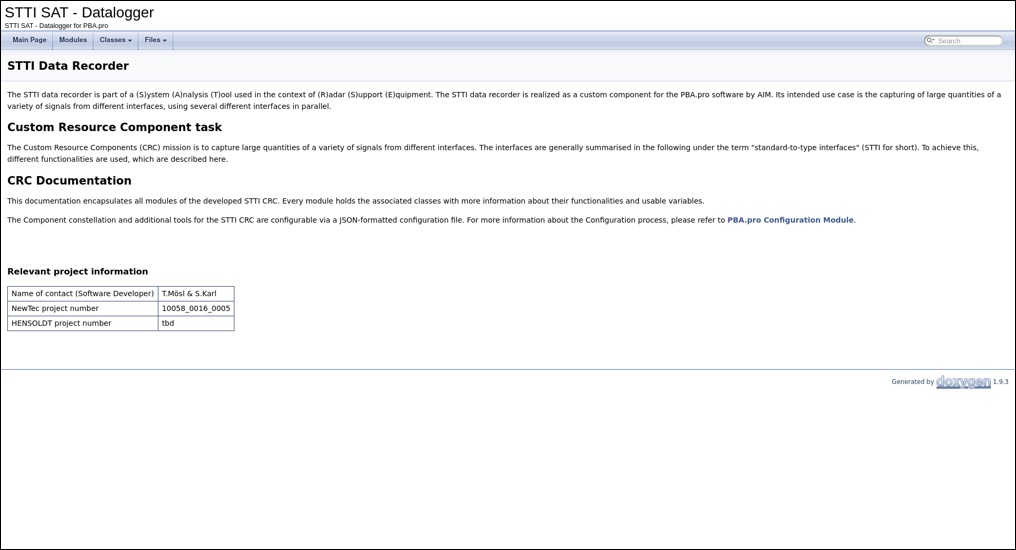
\includegraphics[width=\textwidth]{images/Doxygen_vorher.png}
    \caption{Von Doxygen erzeugte Standarddokumentation}
    \label{fig:doxygen-befor}
\end{figure}
\newpage

\restoregeometry
\section{Gewählter Lösungsansatz} \label{sec:time}
Für die Erstellung eines funktionsfähigen und interaktiven Templates ist eine Integration von JavaScript (JS), Cascading Syle Sheets (CSS) und Hyper Text Markup Language (HTML) 
erforderlich.

\subsection{JavaScript} \label{sec:JS}
JS ist eine objektorientierte Programmiersprache, um dynamische,  bzw. interaktive Elemente auf einer Website zu erstellen \cite{JS_Tutorial}. Dies umfasst in diesem Projekt die Bearbeitung sowie das Kopieren der Codeabschnitte, die Implementierung der Schaltfläche für den Dunkelmodus und den Button zur automatischen PDF-Generierung auf der Website.

\subsection{HTML} \label{sec:HTML}
Um den logischen Aufbau von Webseiten zu realisieren, wird die Auszeichnungssprache HTML verwendet. Durch die Verwendung von Tags können Texte, Bilder, Links und andere Elemente dargestellt werden. Zum Beispiel wird der Text eines Absatzes durch \glqq <p> \grqq{}-Tag eingeleitet oder ein Bild wird durch \glqq <img> \grqq{} dargestellt \cite{HTML_Tutorial}. HTML bildet die Grundlage für Webseiten, auf der CSS und JS aufbauen.

\subsection{CSS} \label{sec:CSS}
CSS ermöglicht die Trennung von Strukturierung und allgemeinem Design. Dabei werden Farben, Schriften, Abstände und Positionen getrennt von der HTML-Struktur behandelt. Durch diese Trennung wird der Code besser organisiert, leichter wartbar und erleichtert Anpassungen \cite{CSS_Tutorial}. Cascading Style Sheets spielen beim sog. Responsive Design eine Schlüsselrolle. Hierbei werden Websiten so gestaltet, dass sie sich an veschiedene Bildschirmgrößen und Auflösungen anpassen könnne \cite{CSS_Responsive_Design}. Der Begriff der Kaskadierung bezieht sich darauf, dass mehrere CSS-Regeln auf ein einzelnes Element angewendet werden können. Sollte dies der Fall sein, so wird die zuletzt definierte Anweisung verwendet \cite{CSS_Tutorial}.

\section{Realisierung}
Doxygen kann entweder mit einer graphischen Benutzeroberfläche, dem \glqq Doxywizard\grqq{}, bedient werden oder über die Kommandozeile. Im Rahmen dieses Projekts konzentrieren wir uns ausschließlich auf die Nutzung der Kommandozeile, um die entsprechenden Fortschritte zu steuern. Um eine Dokumentation generieren zu können, muss ein \glqq Doxyfile\grqq{} vorliegen. Auf Basis dieser Datei werden verschiedene Einstellungen und Optionen festgelegt, die den Dokumentationsprozess beeinflussen. Hierbei handelt es sich um sehr grundlegende Parameter, wie beispielsweise die Entscheidung, ob ein LaTeX Output mit generiert oder in welchem Verzeichnis nach Quelldateien gesucht werden soll.
\begin{figure}[h]
  \centering
  \subfloat[Erstellung des Doxyfile]{
\includegraphics{images/doxygen_init.png}}
  \hfill
  \subfloat[Initialer Run]{
\includegraphics{images/doxygen_first_run.png}}
  \caption{Initialisierung}
  \label{fig:doxygen-init}
\end{figure}

\noindent
Durch die beiden Befehle aus \ref{fig:doxygen-init} wird in dem gewählten Ordner zunächst ein Doxyfile erstellt. Beim anschließenden initialen Durchlauf wird eine Ordnerstruktur generiert. Diese enthält unter anderem den HTML-Output sowie die für die LaTeX-Generierung erforderlichen Dateien.

\begin{figure}[h]
    \centering
    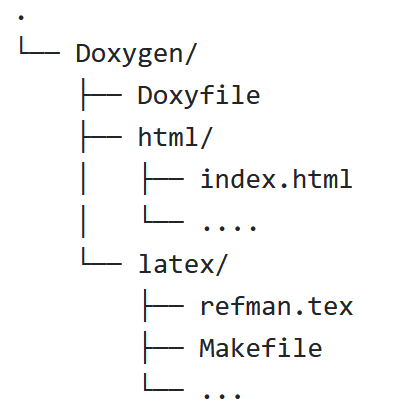
\includegraphics[height=0.35 \textwidth]{images/Tree_view.png}
    \caption{Verzeichnisstruktur nach Ausführen der Befehle aus \ref{fig:doxygen-init}}
    \label{fig:File_Tree}
\end{figure}

\subsection{NewTec-Branding mit CSS und HTML}

Damit das Standarddesign überschrieben werden kann, müssen CSS-Dateien angelegt und als Input im Doxyfile entsprechend deklariert werden, wie bereits in \ref{sec:CSS} erwähnt. Hierbei ist zu beachten, dass die Reihenfolge, in der die Kompilierung stattfindet, eine Rolle spielt: Die zuletzt kompilierte CSS-Datei kann unter Umständen Parameter anderer Dateien wieder überschreiben \cite{CSS_Tutorial}. Um bei der Implementierung strukturiert vorzugehen, bieten sich zwei Ansätze an: Entweder eine große CSS-Datei, die alle Elemente anpasst oder eine fein gegliederte Struktur, in der jede Datei ein ganz bestimmtes Element überarbeitet. In diesem Projekt wurde die erste Variante einer zentralen CSS-Datei umgesetzt. Im Folgenden wird an Hand von Beispielen die Struktur und der Aufbau dieser Datei beleuchtet. Dabei werden spezifische Abschnitte herausgegriffen, um die entsprechenden Anpassungen für einzelne Elemente zu erläutern.
Damit der Benutzer auch nach der Erstellung der Vorlage noch eigene Anpassungen vornehmen kann, wird zu Beginn des Dokumentes ein Bereich definiert, in dem Anpassungen bezüglich der Farbe, des Abstandes oder der Größe von Elementen ohne Gefahr vorgenommen werden können. Außerhalb dieses Bereiches ist es zwar auch möglich, entsprechende Veränderungen vorzunehmen, allerdings birgt dies das Risiko, Abhängigkeiten zwischen Elementen zu beeinträchtigen oder die feste Positionierung so zu verändern, dass das allgemeine Design beeinträchtigt wird. CSS bietet die Möglichkeit eigene Objekte zu definieren, die im gesamten Dokument wiederverwendet werden können. Sie werden entweder mit der \glqq at-rule \grqq{} oder mit einer entsprechenden Syntax verwendet \cite{CSS_Properties} z.B.
\begin{figure}[h]
\centering
\begin{minted}[linenos]{CSS}
        --edit-button-image: url('../images/pencil.svg');  
\end{minted} 
\caption{CSS: Beispiel für ein Objekt}
\label{code:CSS_Example}
\end{figure}

\noindent
Dies ermöglicht es, durch das Umstellen einer Variable mehrere Elemente gleichzeitig zu verändern und somit leichter, das Design anzupassen, ohne erst die Struktur des Codes nachvollziehen zu müssen. Um den Wert des Objekts abrufen zu können wird die CSS-Funktion var() benötigt \cite{CSS_var_funktion}. Ein möglicher Einsatz der Variable aus \ref{code:CSS_Example} sähe folgendermaßen aus:
\begin{figure}[h]
    \centering
    \begin{minted}[linenos]{CSS}
             .editButton {
                background-image:var(--edit-button-image);
                color: white;
                border-color: transparent;
                padding: ...
            }     
    \end{minted}
    \caption{CSS: Verwendung des Objekts aus \ref{code:CSS_Example}}
    \label{code:CSS_Example_Advanced}
\end{figure}

\noindent
Wie in \ref{sec:HTML} erläutert, baut die Verwenung von CSS auf der durch HTML generierten Struktur der Webseite auf. In der Datei \glqq header.html \grqq{} wird dieser Aufbau durch Doxygen generiert. Im Fall von Abbildung \ref{code:CSS_Example_Advanced}:
\begin{figure}[h]
    \centering
    \begin{minted}[linenos]{HTML}
<button id="EditButton" style="height: 20px;"class ="EditButton">
</button>
    \end{minted}
    \caption{HTML Element für \ref{code:CSS_Example_Advanced}}
    \label{code:HTML_Element_für_side_nav}
\end{figure}

\noindent
Das <button>-Element bietet dem Nutzer die Möglichkeit, per Maus oder Tastatur mit der Seite zu interagieren \cite{Button_Element}. In diesem Fall dient es dazu, die Möglichkeit zum Editieren der Codeabschnitte zu aktivieren. Da die jeweilige Dokumentation mehr als einen solchen Abschnitt beinhalten kann, werden alle \glqq EditButton \grqq{} in der gleichnamigen Klasse gekapselt. So wird sichergestellt, dass alle bestehenden Elemente der Gruppe simultan verändert werden können.
Auf dieser Basis werden die Anforderungen \ref{req:Layout} und \ref{req:Notes} umgesetzt. Bei \ref{req:Layout} liegt der Fokus insbesondere auf der Anpassung von Farbcodes. Diese werden von einer firmeninternen Webseite bezogen sowie der Einbindung entsprechender Logos. Die farbliche Hervorhebung von Absätzen baut auf bestehenden, von Doxygen erzeugten Klassen auf, welche so verändert werden, dass eine bessere visuelle Trennung zwischen Code und z.B. Hinweis oder Warnung gegeben ist.
\begin{figure}[h]
    \centering
    \begin{minted}[linenos]{CSS}
        dl.warning {
            background-color: var(--warning-background-color);
            border-color: var(--warning-border-color);
            margin-right: 9px;
            margin-left: 4px;
            border-radius: 5px;
            padding: 5px;
        }
    \end{minted}
    \caption{Angepasste Warnung}
    \label{fig:warning_example}
\end{figure}

\begin{figure}[h]
    \centering
     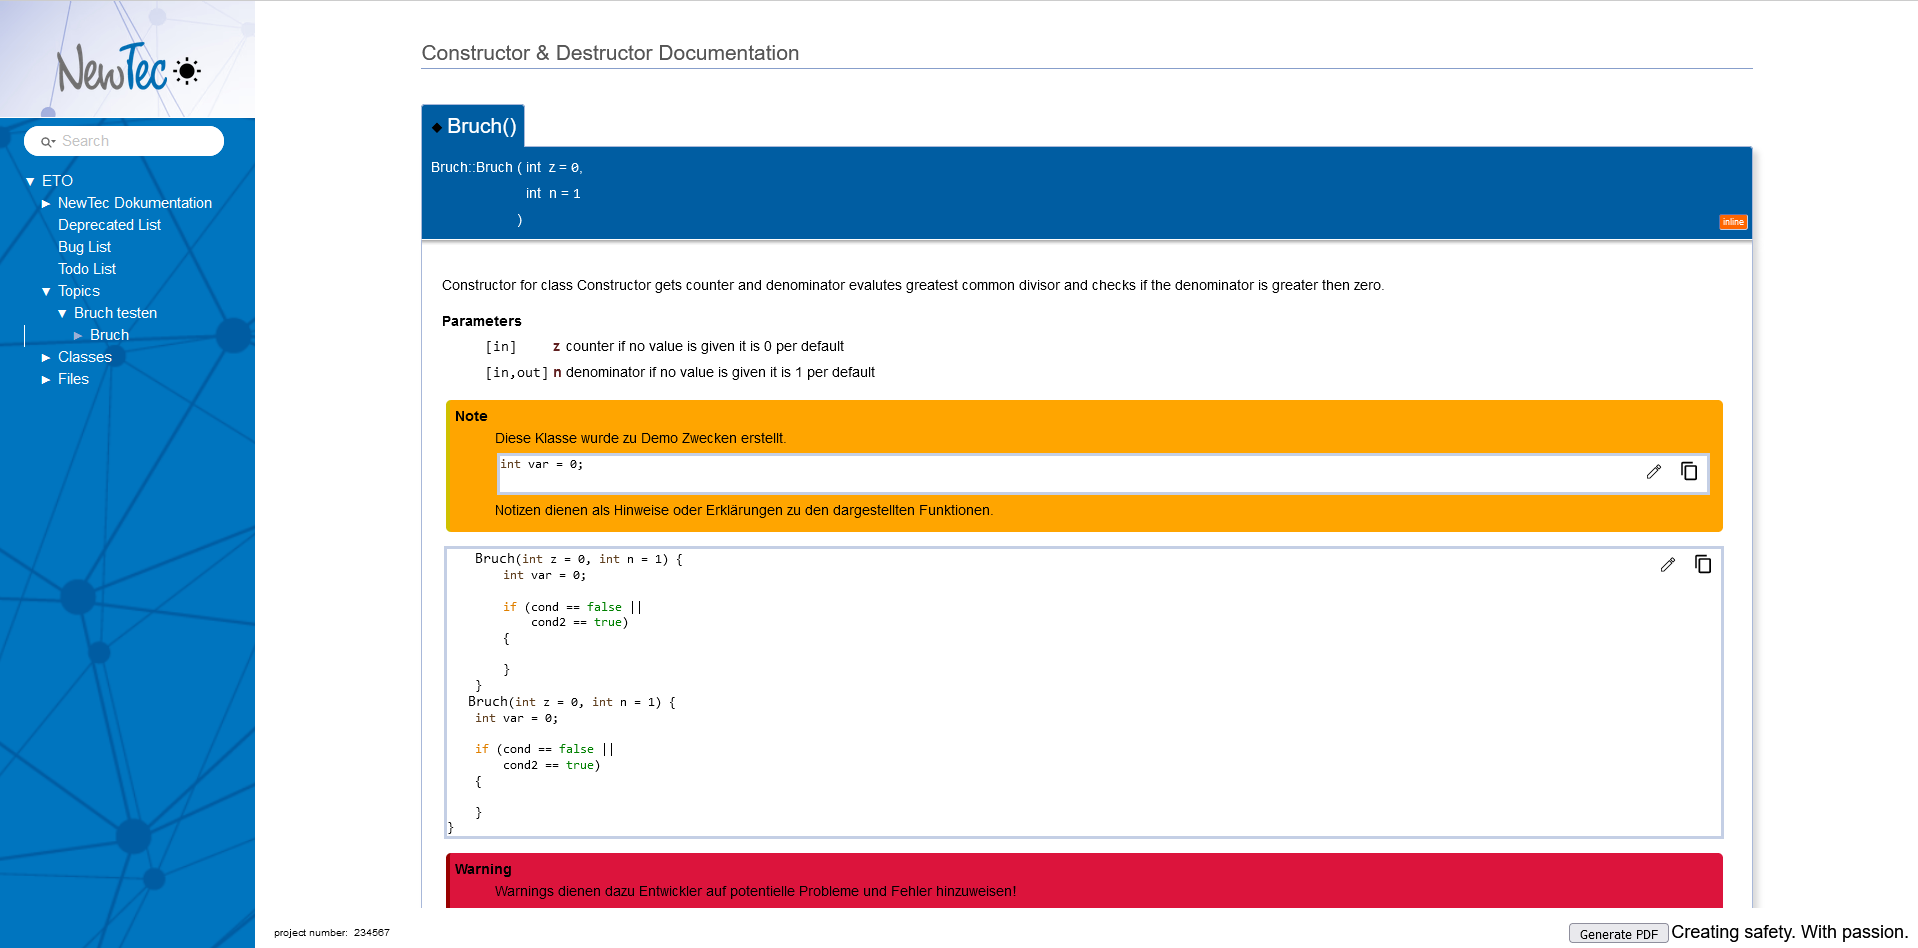
\includegraphics[width=\textwidth]{images/Doxygen_A1undA2_Req.png}
    \caption{Dokumentation nach Umsetzung von \ref{req:Layout} und \ref{req:Notes}}
    \label{fig:doxygen-before}
\end{figure}


\subsection{Integration dynamischer Elemente mit JavaScript}
Das Button-Element aus \ref{code:HTML_Element_für_side_nav} führt standardmäßig keine Aktion aus und bleibt funktionslos. Es kann jedoch ein benutzerseitiges Skript bei bestimmten Ereignissen aufrufen \cite{Button_Element}. Diese werden im folgenden genutzt um \ref{req:Darkmode}, \ref{req:Copy} und \ref{req:PDF} umzusetzen. Um ein Objekt mit dem entsprechenden Skript zu verknüpfen, bestehen zwei Möglichkeiten: Entweder wird in der HTML-Datei das Skript direkt bei den Attributen des Elements oder im Skript selbst wird das Element ausgewählt und \glqq beobachtet \grqq{}. Ein Beispiel für den Prozess des Beobachtens könnte das Warten auf den Druck eines Buttons sein. In diesem Projekt wird die zweite Variante präferiert. Um den Button unabhängig vom Rest des Codes zu halten wird er in einer Klasse gekapselt. Dies bietet auch den Vorteil einer flexibleren Erweiterbarkeit im weiteren Verlauf.
\begin{figure}[h]
    \centering
    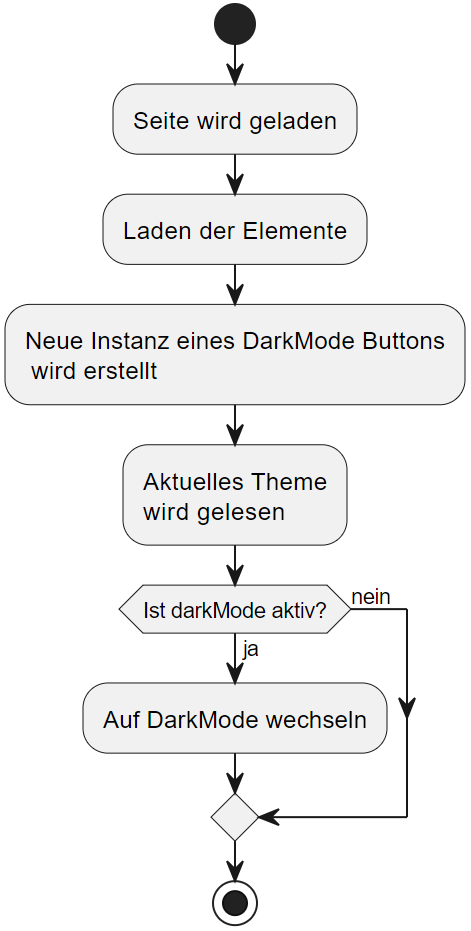
\includegraphics[width=0.3\textwidth]{images/Ini.png}
    \caption{DarkMode-Button Erstellung}
    \label{fig:DarkMode-ini}
\end{figure}

\noindent
Die Bedingungsabfrage aus Abbildung \ref{fig:DarkMode-ini} ist durch das localStorage Objekt möglich. Dieses speichert Wertepaare (Schlüssel/Wert) auch über die Laufzeit des Programms im Browser ab \cite{localStorage_Objekt}. Durch diesen Mechanismus können Werteänderungen, wie die Aktivierung des Dunkelmodus, gespeichert werden. Der Schlüssel \glqq darkMode \grqq{} wird auf \glqq true \grqq{} gesetzt, wenn der Dunkelmodus aktiviert ist, und umgekehrt. Dies ist wichtig, um sicherzustellen, dass das Design bei einem Seitenwechsel innerhalb der Dokumentation konstant bleibt, da jede HTML-Seite neu geladen wird, wenn sie aufgerufen wird. Das \glqq this \grqq{}- Schlüsselwort in JavaScript bezieht sich auf die aktuelle Instanz eines Objekts. Im Kontext des Konstruktors, wie in Abbildung \ref{fig:darkMode_constructor} dargestellt, repräsentiert \glqq this \grqq{} die Instanz des Dunkelmodus Buttons, die erstellt wird. Weiterhin ermöglicht es den Zugriff, die Manipulation sowie die Zuweisung der Attribute und Methoden des Objekts \cite{this_keyword}. Beispielsweise wird in Zeile drei in Abbildung \ref{fig:darkMode_constructor} das \glqq body \grqq{}-Element der HTML-Seite dem Attribut \glqq body \grqq{} der Instanz zugewiesen oder eine Zeile darüber wird das Element mit der ID \glqq darkmode-button \grqq{} ausgewählt und auf das \glqq toggle-button\grqq{}-Attribut gesetzt. Ein zentraler Aspekt für die Funktionalität des Buttons findet sich in Zeile fünf des Konstruktors. Hier wird ein \glqq onclick \grqq{}-Handler für das bereits bestehende \glqq toggle-button\grqq{}-Attribut festgelegt. Wenn der Button gedrückt wird, wird die angegebene Funktion ausgeführt. Die in Zeile sieben aufgeführt \glqq toggle \grqq{}-Funktion teilt sich wiederum in zwei Unterfunktionen auf. Auf der einen Seite ist dies die „toggle-css “ Funktion, die sich auf die Manipulation von CSS-Stilen, einschließlich Hintergrundbilder, Farben und Filtereffekte konzentriert. Auf der anderen Seite steht die \glqq toggle-html \grqq{} Funktion, welche vor allem für das Setzen von globalen Designeinstellungen für das gesamte HTML-Dokument verantwortlich ist. Um einen möglichst genauen Überblick über die Funktionalität der Klasse zu erhalten ist in Abbildung \ref{fig:button_pressed_activity} der Ablauf nach dem Drücken eines Buttons detailliert dargestellt. 

\begin{figure}[h]
    \centering
    \begin{minted}[linenos]{js}
    constructor() {
        this.toggleButton = document.querySelector("#darkmode-button"); 
        this.body = document.body;
        this.darkMode = localStorage.getItem('darkMode') === 'true';
        this.toggleButton.onclick =  () => {
            this.darkMode = this.darkMode ? false : true;
            this.toggle();
            localStorage.setItem('darkMode',this.darkMode);
        };
        this.updateDarkMode();
    }
    \end{minted}
    \caption{Konstruktor des Darkmode Buttons}
    \label{fig:darkMode_constructor}
\end{figure}
\begin{figure}[h!]
    \centering
    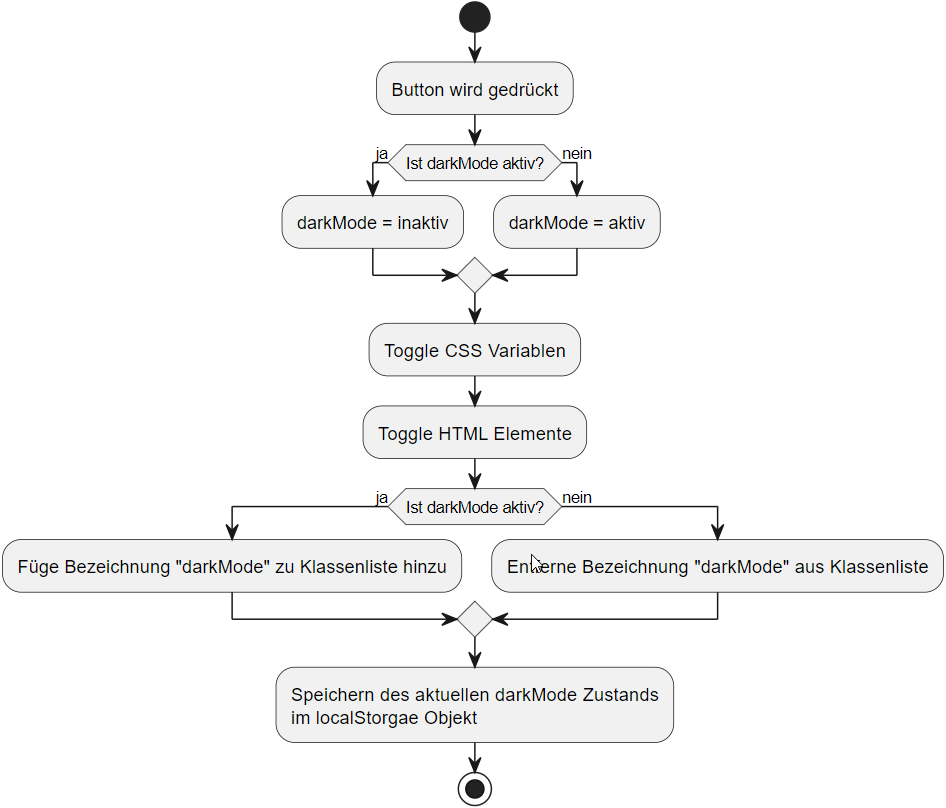
\includegraphics[width=0.85\textwidth]{images/Button_pressed_activity.png}
    \caption{Aktivitätsdiagramm: Button gedrückt}
    \label{fig:button_pressed_activity}
\end{figure}
\newpage
Da der allgemeine Aufbau des Kopier- und Editierbuttons dem des Darkmode-Buttons ähnelt, wird im Folgenden darauf verzichtet, dies im Detail zu beleuchten. Für Leser, die dennoch an einer ausführlichen Beschreibung interessiert sind, finden unter (???) die vollständige Klasse.

\subsection{Generierung eines PDFs mit Node.js und LaTeX}
Für die Realisierung von \ref{req:PDF} reicht JavaScript alleine nicht aus. Das Ausführen von LaTeX-Befehlen und die Erstellung eines PDFs erfordert serverseitige Logik, die aus Sicherheitsgründen nicht direkt im Browser implementiert werden kann. Die Hauptproblematik liegt dabei im beschränkten Zugriff auf das lokale Dateisystem des Geräts, damit das Sicherheitsrisiko minimiert wird. Das direkte Lesen oder Schreiben von Dateien durch JavaScript im Browser kann Sicherheitslücken aufreißen. Um die Funktionalität trotzdem umsetzten zu können, ist eine serverseitige Umgebung wie Node.js notwendig. Bei Node handelt es sich nicht um ein Framework oder eine Bibliothek sondern um eine Laufzeitumgebung \cite{Syed}. Das bedeutet es stellt eine vollständige Plattform dar, die es ermöglicht serverseitige Anwendungen zu erstellen. Diese bietet die Möglichkeit, JavaScript auf dem Server auszuführen, wodurch Befehel, die das Dateisystem betreffen, sicher ausgeführt werden können \cite{Syed}. 

\noindent
In diesem Projekt wird ein lokaler Webserver der \glqq localhost \grqq{} genutzt, um die erforderlichen Befehle auszuführen. Durch diese Architektur kann der Button eine Anfrage an den Node.js-Server senden. Dieser ist in der Lage, auf das System zuzugreifen und entsprechende Informationen oder, wie in diesem Fall, Dokumente an den Browser zurück zu senden. Node stellt bereits standardmäßig viele Module bereit, um den erforderlichen Webserver aufzusetzen.

\begin{figure}[H]
    \begin{minted}[linenos]{js}
                const http = require('http');
                const fs = require('fs');
                const path = require('path');  
    \end{minted}
    \centering
    \caption{Import der Module}
    \label{code:Import_Module}
\end{figure}

\noindent
Die Module aus Abbildung \ref{code:Import_Module} werden für die Erstellung des HTTP-Servers, das Lesen von Dateien und die Arbeit mit Dateipfaden verwendet. Das \glqq http \grqq{}-Modul enthält die Funktion \glqq createServer \grqq{}. Diese gibt eine Instanz eines Serverobjekts zurück. Diese Instanz wird verwendet, um auf eingehende HTTP-Anfragen zu reagieren. Als Argument wird der Funktion eine Callback-Funktion übergeben, diese wird jedes Mal ausgeführt, sobald eine Anfrage an den Server gesendet wird. In diesem Callback-Block wird die eigentliche Server-Logik implementiert. Die Callback-Funktion hat zwei Parameter, einerseits \glqq req \grqq{} für die Anfrageinformationen und andererseits \glqq res \grqq{} für die Antwort an den Client (Browser). Abhängig von der angeforderten URL gibt der Server unterschiedliche Antworten zurück.

\begin{figure}[H]
    \centering
    \begin{minted}[linenos]{js}
const server = http.createServer((req, res) => {
 if (req.url === '/PDF') {
        const pdfFilePath = path.join(__dirname, '../latex/refman.pdf');

        fs.readFile(pdfFilePath, (err, data) => {
            if (err) {
                console.error('Error reading PDF file:', err);
                res.statusCode = 500;
                res.end('Internal Server Error');
            } else {
                res.setHeader('Content-Disposition', 'filename=file.pdf');
                res.setHeader('Content-Type', 'application/pdf');
                res.end(data);
            }
        });
    } else {
        res.end(server.statusCode);
    }
});
const PORT = 5000;
server.listen(PORT, () => {
});
    \end{minted}
    \caption{Callback und starten des Servers}
    \label{code:Callback}
\end{figure}
\noindent
Hierbei führt die URL \glqq /PDF \grqq{} (Abbildung \ref{code:Callback} Zeile 2) dazu, dass die Logik für den PDF-Download ausgeführt wird. Für alle anderen Anfragen erhält der Client eine generische Antwort, die den aktuellen Status des Servers widerspiegelt. Der Server wird erfolgreich gestartet und horcht auf einem vordefinierten Port, um eingehende Anfragen zu verarbeiten.

\noindent
Dieses Vorgehen trifft die Annahme, dass ein entsprechendes PDF bereits im Dateisystem existiert. Um diese Grundlage zu schaffen bestehen zwei Möglichkeiten: Entweder wird das PDF bei der Dokumentationsgenerierung durch Doxygen miterzeugt oder wenn die entsprechende URL-Anfrage vom Server verarbeitet wird. Auf Grund von besserer Effizienz, Doxygen erzeugt die erforderlichen \glqq Tex\grqq{}-Dateien automatisch als Teil des Build-Prozesses sowie zur Vermeidung der Übernahme nicht gewollter Dokumentationsbausteine, wird die erste Variante realisiert. Da die Projekte zum Testen des Tools in einer \glqq Linux \grqq{} Umgebung aufgesetzt sind, wird im folgenden die Vorgehensweise anhand dieser Umgebung vorgestellt. Diese lässt sich nahtlos auf die Version für \glqq Windows \grqq{} übertragen.

\noindent
Da der Aufwand dem bestehenden Doxygen Tool weitere Flags hinzuzufügen den Rahmen dieses Projektes sprengen würde, wird stattdessen ein eigenes Schlüsselwort definiert. Dieses nutzt Doxygen, um die enstprechenden Generierungen durchzuführen und fügt an den geeigneten Stellen die Befehle zum Starten des Servers sowie zur PDF Generierung ein. Um eine Ausführung aus jedem Verzeichnis zu ermöglichen (ohne immer den kompletten Skript Pfad angeben zu müssen), muss das Skript in der Datei \glqq ~/.bashrc \grqq{} geschrieben werden. Diese enthält Befehle und Einstellungen, die für die Umgebung relevant sind. Daher wird sie beim Starten der Shell ausgeführt. Dieser Mechanismus stellt sicher, dass das Skript bereits global in der Umgebung bekannt ist und aufgerufen werden kann.

\noindent
Für eine bessere Übersichtlichkeit wird außerdem eine Manpage erstellt, in der können alle Befehle, Flags und weitere Optionen nachgelesen werden. Generell können alle Befehle von Doxygen ausgeführt werden. Damit der PDF-Button jedoch vollumfänglich genutzt werden kann, muss die Dokumentation mittels des Schlüsselwort \glqq doxy + Doxyfile \grqq{} generiert werden.

\begin{figure}[H]
    \begin{minted}[linenos]{bash}
doxy(){
if [ -f "$1" ]; then
        if command -v node &> /dev/null; then
                if [ "$2" == "-s" ]; then
                        doxygen $1
                        node ./doxygen/js/server.js &
                        NODE_PID=$!
                fi
                if [ "$2" == "-st" ]; then
                        kill NODE_PID
                fi

        else
                echo "Node is not installed"
        fi
else
        doxy man
fi
}
    \end{minted}
    \centering
    \caption{Command Line Tool \glqq doxy \grqq{}}
    \label{code:doxy_command_line}
\end{figure}

\section{Zusammenfassung}

Die Entwicklung des Templates ermöglicht es den Benutzern, Dokumentationen in einem zeitgemäßen und individuell angepassten Branding zu erstellen. Durch die Integration verschiedener Funktionen wie einem Darkmode-Button und der Möglichkeit, Code-Abschnitte zu bearbeiten und zu kopieren oder PDFs direkt erzeugen zu können wird die Erstellung von Dokumentationen vereinfacht und bietet eine Möglichkeit zur Personalisierung. Die Abbildung \ref{fig:Template_Final} veranschaulicht das endgültige Template mit all diesen Anpassungen und Funktionen, das eine effiziente und maßgeschneiderte Dokumentation im NewTec-Stil ermöglicht.

\begin{figure}[H]
    \centering
    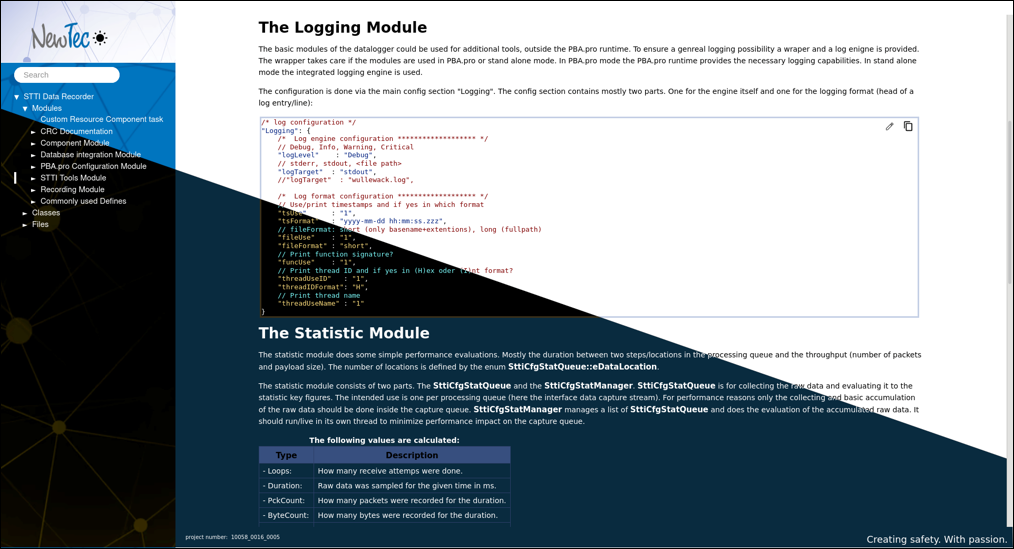
\includegraphics[width = 1.1\linewidth]{images/Finale_Doku.png}
    \caption{Finales Template}
    \label{fig:Template_Final}
\end{figure}






\chapter{
Implementierung einer Schnittstelle zwischen MS Project und MS Excel im PDCA Planner
} \label{chap:sling}
Um eine effektive Projektplanung in der heutigen, schnelllebigen Arbeitswelt zu gewährleisten, sind unterstützende Projektmanagement-Tools von zentraler Bedeutung. Im Kontext der Bachelorarbeit  \glqq Entwicklung eines PDCA-Projektmanagement-Workflows in Microsoft Office \grqq{} liegt der Fokus auf der Erstellung einer Schnittstelle zwischen MS Project und MS Excel innerhalb des erstellten Tools. Die Schnittstelle zielt darauf ab die Vorteile beider Tools zu vereinen, einerseits die detaillierte Projektplanung in MS Project und andereseits die flexible Datenaufbereitung und -analyse in MS Excel.


\section{Allgemeines}


\subsection{PDCA Planner}

Der bereits entwickelte Planner beruht auf dem PDCA-Zyklus auch Deming-Rad oder Deming-Kreis genannt dieser ermöglicht eine kontinuierliche Verbesserung von Prozessen und Abläufen. Der Aufbau umfasst die vier Schritte Plan, Do, Check und Act \cite{Syska}. Durch die zyklische Wiederholung dieser Schritte sollen auf lange Sicht die Effizienz gesteigert und Fehler reduziert werden. Hierbei ist wichtig zu beachten, dass es zielführender ist, viele kleine Schritte vorzunehmen, anstatt alles in einem Durchlauf verbessern zu wollen \cite{Syska}. Der Zyklus besitzt kein definiertes Ende, sonder legt die Grundlage für einen kontinuierlichen Prozess der Anpassung beziehungsweise Verbesserung. Um einen besseren Überblick über dieses Modell zu ermöglichen, ist in \ref{fig:PDCA-Zyklus} ein Durchlauf anhand eines alltäglichen Beispiels dargestellt.\newpage

\begin{figure}[h]
    \centering
    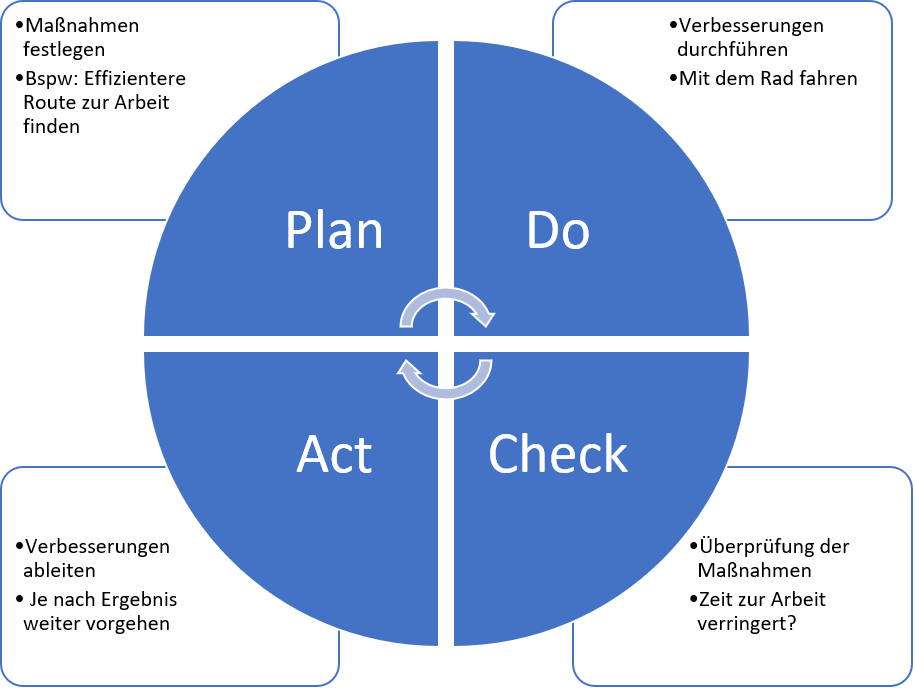
\includegraphics[width= \textwidth]{images/PDCA_Zyklus.png}
    \caption{PDCA-Zyklus}
    \label{fig:PDCA-Zyklus}
\end{figure}

\noindent
Der PDCA Planner abstrahiert den Kreislauf in einer Anwendung, die in MS Excel implementiert ist. Er ermöglicht die Erfassung, Analyse und zusammengefasste Darstellung von projektbezogenen Informationen. Dadurch wird beispielsweise ein detaillierter Vergleich zwischen Soll-und Istwert des Budgetverbrauchs oder eine genaue Messung des Projektfortschritts möglich. Die benötigten Daten werden aus zwei verschiedenen Datenbanken bezogen: In einer werden spezifische Mitarbeiterdaten sowie Stundenbuchungsdaten gespeichert, während die andere Informationen wie beispielsweise Daten des PDCA-Planners oder spezifischere Projektdaten enthält. Zusätzlich dazu gibt es noch eine weitere als Tabellenblatt realisierte interne Datenbank, diese fungiert einerseits als Grundlage für die Darstellung der importierten Daten, andererseits als Backup falls der Benutzer Daten in der Oberfläche ungewollt löschen oder verändern sollte. Der Planner bietet zwei verschiedene Modi für die Projektdarstellung, deren Detailgrad variiert. Da diese Features für die Funktionalität der Schnittstelle nicht relevant sind, werden diese nicht tiefergehend erläutert.

\subsection{MS Project}
Microsoft Project ist eine Projektmanagement-Software, die ein breites Spektrum an Tools zur Planung, Verwaltung und Überwachung von Projekten bietet. Mit der Fähigkeit, Start- und Endtermine zu erfassen, ermöglicht die Software Benutzern, detaillierte Zeitpläne für jeden Arbeitsschritt zu erstellen und zeitliche Abhängigkeiten zwischen Aufgaben festzulegen \cite{MSProject}. Diese Herangehensweise ermöglicht es, Projekte detaillierter zu strukturieren. Durch die Integration dieser Daten in den PDCA Planner wird der zeitliche Aspekt nahtlos in den Gesamtkontext des Projekts eingebunden, wodurch eine verlustfreie Koordination gewährleistet wird.

\section{Anforderungsanalyse und Definition der Schnittstellenparameter}

Der PDCA Planner wurde ausschließlich mithilfe der Programmiersprache \glqq Visual Basic for Application \grqq{} (VBA) implementiert, wobei die in MS Office-Anwendungen integrierte  Entwicklungsumgebung verwendet wurde. VBA ist eine objektorientierte Sprache, die speziell für die Steuerung von Office-Anwendungen entwickelt wurde. Sie ermöglicht die Automatisierung von Prozessen und den Transfer von Daten zwischen verschiedenen Office-Anwendungen \cite{Kogan}. Um eine möglichst große Kompatibilität zu schaffen, wird ein Großteil der Schnittstelle ebenfalls in VB geschrieben werden. Dies führt zu  einem geringeren Entwicklungsaufwand, da zum Beispiel Module aus dem PDCA Planner direkt verwendet werden können. Jedoch stellt die Python-Bibliothek \glqq OpenPyXL \grqq{} eine sehr flexible und plattformunabhängige Alternative zu VBA dar. Sie ermöglicht das Lesen und Schreiben von Excel-Dateien, genauso wie das Bearbeiten von Zellen und Tabellen. Aus diesem Grund wird die Schnittstelle als Symbiose dieser beiden Programmiersprachen entwickelt.

\noindent
Eine der grundlegenden Anforderungen an die Schnittstelle ist die bidirektionale Datenübertragung. Dies bedeutet, dass Daten problemlos zwischen dem PDCA Planner und einer MS Project-Datei kopiert, bearbeitet und nahtlos wieder in den Planner integriert werden können. Im Hinblick auf die erforderlichen Python-Dateien soll der Planner als eigenständiges Dokument konzipiert bleiben und nicht von einer Ordnerstruktur umgeben sein. Dadurch wird eine einfachere Handhabung sowie eine verlässlichere Funktionalität gewährleistet. Im Planner werden Projekte in Positionen und Arbeitspakete unterteilt. Positionen beschreiben größere Teile des Gesamtprojekts und werden wiederum in mehrere Arbeitspakete gegliedert. Diese Struktur lässt sich auf die MS Project-Datei übertragen. In dieser wird ein Projekt in Sammelaufgaben(Positionen) unterteilt. Eine Sammelaufgabe kann wiederum mehrere Unteraufgaben(Arbeitspakete) beinhalten aber auch weitere übergeordnete Aufgaben. Es ist jedoch ratsam, das Hinzufügen einer weiteren Hierarchieebene zu vermeiden, da der Planner selbst nur bis zu einer Tiefe von vier Ebenen (zum Beispiel 1.1.1.1) darstellen kann. Außerdem ist die Anzahl an Positionen konstant. Diese werden für die Erfassung geleisteter Stunden genutzt und neu hinzugefügte können nicht in die Datenbank zurückgespiegelt werden. Eine weitere wichtige Voraussetzung für einen reibungsloseren Export/Import besteht darin, dass der Projektplanungsprozess vollständig in MS Project durchgeführt wird und nicht zwischen beiden Seiten aufgeteilt wird. Das bedeutet Arbeitspakete sollten nur in MS Project hinzugefügt oder bearbeitet und dann in den Planner integriert werden.

\begin{figure}[H]
    \centering
    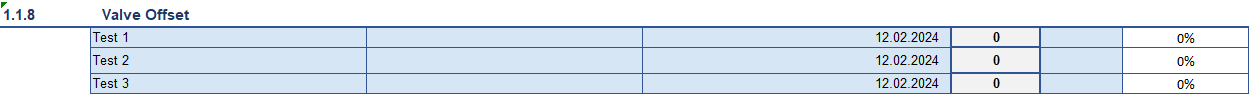
\includegraphics[width=\linewidth]{images/Excel_Position_Beispiel.png}
    \caption{Position mit Arbeitspaketen im PDCA Planner}
    \label{fig:PDCA_Example}
\end{figure}


\section{Entwicklung der Schnittstelle}
In VBA wird zwischen einer Subroutine (Sub) und einer Funktion unterschieden. Es gibt zwei wesentliche Unterschiede:
\begin{enumerate}
    \item Rückgabewert: Eine Funktion gibt im Gegensatz zu einem Sub einen Wert zurück.
    \item Generelle Verwendung: Funktionen werden in VBA häufig dazu verwendet Berechnungen durchzuführen oder Werte zu initialisieren. Sub's hingegen dienen dazu bestimmte Aufgaben oder Aktionen wie zum Beispiel das Öffnen von Dokumenten oder das Aktualisieren von Datenbanken durchzuführen. Ebenso kann ein Sub mit einem Button aus der Benutzeroberfläche verknüpft werden, dies ist mit Funktionen nicht möglich.
\end{enumerate}
In diesem Projekt werden Sub's eine tragende Rolle spielen, da diese auch über Python aufgerufen werden können und daher den Austausch der Daten starten können.


\subsection{Realisierung mit VBA}
Die Softwarearchitektur kann in drei Hauptkomponenten aufgeteilt werden: Die zentrale Subroutine zur Steuerung des allgemeinen Ablaufs, Funktionen und Subs um eine Verbindung mit der internen Datenbank aufzubauen beziehungsweise deren Status abzurufen und ein Modul für die Integration der Python-Skripte. Um eine klare Unterscheidung zwischen den verschiedenen Elementen zu ermöglichen, werden eindeutige ID's für Positionen und Arbeitspakete sowohl im Planner als auch in MS Project verwendet. Im Folgenden werden diese Komponenten detaillierter beleuchtet.

\begin{enumerate}
    \item Zentrale Subroutine: Die \glqq Transfer \grqq{}- Subroutine ist verantwortlich für den Austausch von Daten zwischen MS Excel und MS Project. Sie wird vom entsprechenden Python Modul aufgerufen und empfängt Daten von diesem. Der Planner wurde in mehrere separate Module unterteilt, wobei für jedes Modul eine eigene Klasse definiert wurde. Diese Struktur zu verstehen ist in VBA essentiell, da es sich wie bereits erwähnt um eine objektorientierte Programmiersprache handelt. Durch die Klassenstruktur wird das Verständnis der Subroutine erleichtert. Zunächst erfolgt die Deklaration verschiedener Variablen und Objekte, darunter Instanzen von Klassen wie \glqq clsPDCAPosition\grqq{} (für die Darstellung einer Position) und \glqq clsWorkPackage\grqq{} (für die Repräsentation eines Arbeitspakets). Zudem wird eine Instanz des Datenbankverbindungsmoduls (\glqq ModInternDatabaseConnector\grqq{}) erstellt. Um sicherzustellen, dass keine Datenübertragung auf bereits gelöschte Elemente stattfindet wird die Funktion \glqq wasDeleted \grqq{} aufgerufen. Dies löscht nicht mehr vorhandene MS Project-IDs aus den zu übertragenden Daten heraus. Die Hauptschleife der Routine iteriert über ein Array von Schlüsselwerten. Diese repräsentieren eine spezifische Nummerierung innerhalb von MS Project, die als \glqq Gliederungsnummerierng \grqq{} bekannt ist. Ein Beispiel hierfür wäre beispielsweise \glqq 1.1.2 \grqq{} oder \glqq 3.1 \grqq{}. Während jedes Durchlauf wird die zugehörige Nummer an die Funktion \glqq EvalDepth \grqq{} übergeben, um die Tiefe des aktuellen Datenpakets zu bestimmen. Anhand der ermittelten Tiefe wird eine Fallunterscheidung durchgeführt, wenn diese 1 oder 2 beträgt, wird die entsprechende Position im Projektbaum identifiziert und aktualisiert oder neu gesetzt. Sollte die Tiefe 3 betragen, wird überprüft, ob das Arbeitspaket bereits existiert. Falls nicht, wird es erstellt, ansonsten werden die Werte auch hier aktualisiert, um sicherzustellen, dass sie auf dem neuesten Stand sind. Am Ende wird das Arbeitsblatt für eine einheitliche Ansicht entsprechend der Vorgaben formatiert. Eine kompakte Darstellung dieser Subroutine ist unter \ref{fig:activity_transfer} zu finden.
    \item Datenbankverbindung: Dieses Modul beinhaltet eine Sammlung von Funktionen und Subroutinen, die darauf abzielen Daten aus der internen Datenbank zu beziehen und zu aktualisieren. Die Funktionen \glqq getPackage \grqq{} und \glqq getPosition \grqq{} verfolgen ein ähnliches Ziel mit ähnlichem Prinzip und stehen beispielhaft für dieses Modul. Beide beziehen über eine Methode der Datenbankklasse die aktuellen Position- beziehungsweise Arbeitspaketdaten. Als Filterparameter wird die aktuelle ID an diese Funktionen übergeben. Wenn diese mit einer in den aktuellen Daten übereinstimmt, wird der entsprechende Eintrag zurückgegeben. Das Modul enthält viele weitere Funktionen, die auf ähnliche Weise wie die zuvor erläuterten implementiert sind. Da ihr Aufbau und Funktionsweise weitestgehend vergleichbar sind, werden diese hier nicht im Detail behandelt. Stattdessen sind sie Teil eines größeren Systems, das in \ref{fig:Database_modul}
    detailliert dargestellt ist.
\end{enumerate}
\begin{figure}[H]
    \centerline{\includesvg[width=1.35\columnwidth]{images/DatabaseConnector.svg}}
    \caption{Modul für die Datenbankverbindung}
    \label{fig:Database_modul}
\end{figure}

\begin{enumerate}\addtocounter{enumi}{2}
     \item Integration von Python-Skripten: Die beschriebene Subroutine zur Steuerung des Datenaustausch wird direkt von einem Python-Modul aufgerufen, um Daten zu empfangen und zu verarbeiten. Da wie bereits erwähnt der Planner als einzelne Datei ohne umgebende Ordnerstruktur funktionieren soll muss eine solche Struktur anderweitig bereitgestellt werden. Hierfür wird die in \ref{sub:Doxygen} erläuterte Webplattform GitHub verwendet, genauer gesagt der Prozess des Klonens. Dieser ist ein Mechanismus, der es Benutzern ermöglicht, eine exakte Kopie eines Repositorys auf ihren lokalen Computer herunterzuladen \cite{git_clone}. Dies geschieht durch Ausführen des Befehls \glqq git clone \grqq{} in der Befehlszeile oder im Terminal, gefolgt von der URL des Repositorys, das geklont werden soll.
    Dadurch können Nutzer lokal an einem Projekt arbeiten, Änderungen vornehmen und eigene Beiträge hinzufügen, bevor sie diese wieder auf GitHub hochladen \cite{git_clone}.

    \noindent
    VBA bietet die Möglichkeit, externe Anwendungen und Skripte über das Windows Script Host-Objektmodell zu steuern \cite{shell_objekt}. 
    \begin{figure}[H]
        \centering
        \begin{minted}[linenos]{js}
    Set objShell = CreateObject("WScript.Shell")
    command = GitRepoURL & scriptFolderPath
    shell.Run command, 0, True
        \end{minted}
    \caption{Erstellung eines Shell Objekt und klonen des Repository}
    \label{code:WScript.shell}
    \end{figure}

    \noindent
    In \ref{code:WScript.shell} wird ein Objekt dieser Klasse instanziiert. Dieses Objekt ermöglicht den Zugriff auf verschiedene Funktionen des Betriebssystems über die Windows-Shell. Mit Methoden wie \glqq Run \grqq{} können Befehle ausgeführt werden, was insbesondere nützlich ist, um Systembefehle oder externe Programme direkt aus einem Skript heraus zu starten \cite{shell_objekt}. Diese Funktionalität wird genutzt, um ein Setup für die Ordnerstruktur zu erstellen. Eine Setup-Routine wird implementiert, die mithilfe des Objekts aus \ref{code:WScript.shell} einen Ordner names \glqq Script \grqq{} auf Benutzerebene erstellt. In diesen Ordner wird dann mittels des oben genannten Befehl das  Repository \glqq PDCA\grqq{} geklont. Durch diese Schritte wird die Möglichkeit geschaffen, die gewünschten Python-Skripte per Code an eine vorgegebene Stelle zu kopieren.

    \noindent
    Um diese ausführen zu können muss auf dem jeweiligen Rechner Python installiert sein. Da vor allem bei der Installation auf Windows ein paar Dinge beachtet werden müssen, wird als Hilfestellung eine Anleitung geschrieben, um die Schnittstelle vollumfänglich nutzen zu können. Der wichtigste Punkt ist hierbei das Hinzufügen des Speicherortes der Python Executable zu den Systemumgebungsvariablen. Sollte dies nicht geschehen so können die Skripte zum Datentransfer nicht ausgeführt werden. Beispielsweise wird auch eine Funktion geschrieben, die nach dem Pfad zur Python-Executable sucht und diesen an die aufrufende Funktion zurückgibt. Dafür wird nach dem gleichen Prinzip wie beim Klonen vorgegangen, allerdings nun mit dem Befehl \glqq where python \grqq{}. Dieser kann nur einen absoluten Pfad ausgeben, wenn die entsprechende Umgebungsvariable existiert.
  \end{enumerate}

\begin{figure}[H]
    \centerline{\includesvg[width=0.75\columnwidth]{images/transfer.svg}}
    \caption{Aktivität des Transfer-Sub}
    \label{fig:activity_transfer}
\end{figure}



\subsection{Realisierung mit Python}

Python bietet einige Vorteile gegenüber VBA aber auch anderen Programmiersprachen. Neben der Einfachheit und Vielseitigkeit besitzt Python auch eine sehr große Standardbibliothek um verschiedenste Aufgaben zu lösen. Sollte diese nicht ausreichen gibt es die Möglichkeit aus einer breiten Palette aus Bibliotheken und Frameworks seine Installation zu erweitern. Neben der bereits angesprochenen \glqq OpenPyXL \grqq{}-Bibliothek wird häufig auch die Bibliothek \glqq Pandas \grqq{} verwendet, um Daten zu analysieren und zu manipulieren. Sie bietet zwei hauptsächlich genutzte Datenstrukturen, Series und DataFrames. Eine Series ist eine eindimensionale Datenstruktur, welche eine Liste oder Array von Werten enthält. Währendessen ein DataFrane eine tabellarische Datenstrukur ist, die aus Zeilen und Spalten besteht und eine große Menge an Daten in einem zweidimensionalen Format darstellen kann. Da ein Excel-Sheet ebenfalls eine Struktur aus Zeilen und Spalten aufweist, können diese Daten in einen DataFrame überführt und analysiert beziehungsweise manipuliert werden.

\noindent
Die Aufgaben werden unter den drei Skripten \glqq export.py\grqq{}, \glqq import.py \grqq{} und \glqq kopieren.py\grqq{} aufgeteilt. Die ersten beiden sind für den jeweiligen Export beziehungsweise Import der Daten verantwortlich, ein weiteres erstellt eine Arbeitskopie einer Project-Datei. Einerseits sorgt dies für einen einheitlichen Arbeitsablauf, da auch beim Planner zunächst eine Kopie erstellt werden muss, andererseits ist das Erstellen einer Kopie unerlässlich, da die implementierten Subs immer nur in der Basis-Datei beziehungsweise Kopien von dieser vorhanden sind. Ohne eine solche Kopie müsste für jede neue Aufgabe ein erneuter Download durchgeführt werden. Da der PDCA-Planner die zentrale Komponente darstellt erfolgt die Namensgebung der Dateien aus Sicht von Excel. Das bedeutet der Datentransfer von Excel nach Project stellt einen Export dar, während das Gegenstück von Project nach Excel einen Import repräsentiert.

\noindent
Für einen besseren Überblick ist in \ref{fig:komponenten} eine komplette Darstellung der Komponenten und deren Interaktionen untereinander. Mit Hilfe dieser werden im folgenden die Funktionen der Python-Skripte näher erläutert. Zu Beginn des Arbeitsflusses, bevor Daten exportiert werden können, muss die oben erwähnte Kopie erzeugt werden. Hierzu wird die entsprechende Subroutine \glqq Copy \grqq{} in MS Project aufgerufen, diese wiederum ruft über eine in VBA geschriebene Funktion das Python-Skript auf. Zunächst wird jedoch die bereits beschrieben Setup-Routine durchgeführt, erst dann wird das Skript gestartet.

\noindent
Da für dieses Projekt die Standardbibliothek nicht ausreicht, müssen noch zusätzliche Bibliotheken installiert werden. Darunter \glqq pandas \grqq{} zur Datenverarbeitung, \glqq pytz \grqq{} für das Arbeiten mit Kalenderdaten, \glqq pywin32 \grqq{} um MS Project und MS Excel Dateien zum Bearbeiten öffnen zu können und die Bibliothek \glqq OpenPyXL \grqq{}. Um dies automatisiert durchführen zu können wird das \glqq subprocess \grqq{}-Modul benötigt. Es ermöglicht, externe Prozesse zu erstellen, auszuführen und mit ihnen zu interagieren. Vereinfacht stellt es eine Schnittstelle zur Kommunikation mit dem Betriebssystem dar, um entsprechende Befehle auszuführen. Für die Installation wird der \glqq pip install \grqq{}-Befehl benötigt \cite{pip_command}. Pip ist ein Packet Manager für Python, wird er über die Kommandozeile aufgerufen sucht er standardmäßig auf PyPI (Standard-Repository für Python-Pakete) nach der Bibliothek und deren Abhängigkeiten \cite{pip_command}.

\begin{figure}[H]
    \centering
    \begin{minted}[linenos]{python}
def install(package):
subprocess.check_call([sys.executable, "-m", "pip", "install", package])
    \end{minted}
    \caption{Installation der benötigten Bibliotheken}
    \label{fig:install_package}
\end{figure}

\noindent
Damit nicht nur ein Paket installiert werden kann, wird ein Array mit den oben genannten Paketen definiert und in einer Schleife für jeden Eintrag die install-Funktion aufgerufen. Das Modul zum Kopieren erzeugt daraufhin die Arbeitskopie an einem gewünschten Speicherort.
\begin{figure}[H]
    \centerline{\includesvg[width=1.35\columnwidth]{images/Component.svg}}
    \caption{Interaktion der Komponenten untereinander}
    \label{fig:komponenten}
\end{figure}

\noindent
Das Export- und Importmodul ähnelt sich in einem Großteil des Ablaufs. Daher wird im Folgenden nur das Exportmodul behandelt. Wie in \ref{fig:export_module} dargestellt, erhält das Skript zwei Argumente, um zwischen einer Aktualisierung bestehender Daten und einer erstmaligen Exportierung eines Worksheets zu unterscheiden. Diese Information wird mit dem zweiten Argument übergeben, mm auf die zu exportierenden Daten zugreifen zu können, wird zuerst der Pfad zur entsprechenden Excel-Datei übermittelt.

\noindent
Im Falle einer Aktualisierung werden zunächst Variablen wie beispielsweise die Position der Projektdaten in der Datenbank oder das Startdatum des Projekts initialisiert. Daraufhin wird das Worksheet geladen und in einer Schleife überprüft, ob sich die Daten geändert haben. Wenn Änderungen festgestellt werden, werden die entsprechenden Einträge aktualisiert. Diese wird so lange durchlaufen, bis keine weiteren Daten vorhanden sind.

\noindent
Die initialen Schritte sind im Falle eines erstmaligen Exports identisch, jedoch werden vor der Hauptschleife noch die Ressourcen aus dem Planner übernommen. Bei diesen handelt es sich in den meisten Fällen um Personen die als Arbeitsressource eingeplant werden können. MS Project unterscheidet zwischen drei Arten dieser Ressourcen, einer Unternehmensressourcen, Nicht-Unternehmensressourcen oder Generischen Ressource \cite{project_ressource}. In diesem Projekt werden Nicht-Unternehmensressourcen angelegt, der Unterschied zu den Unternehmensressourcen liegt darin, dass diese nur lokal angelegt werden und nicht alle Benutzer auf diese zugreifen können. Nach dem Anlegen wird aus der wöchentlichen Arbeitszeit, welche im Planner hinterlegt ist, noch die \glqq Max-Units \grqq{}-Variable der Ressourcen berechnet. Diese gibt an wie viel Prozent der in Project definierten Wochenarbeitszeit eine Person eingesetzt werden kann.

\noindent
In der Hauptschleife wird überprüft, ob es sich um eine Sammelaufgabe handelt. Dies wird durch einen Vergleich der \glqq Tiefe \grqq{} von vorangegangener, aktueller und nächster Aufgabe ermittelt. Falls ja wird diese dem Project hinzugefügt. Andernfalls wird die Aufgabe zur aktuellen Sammelaufgabe hinzugefügt. Auch hier wird die Schleife solange durchlaufen, bis keine weiteren Daten vorhanden sind.
\begin{figure}[H]
    \centerline{\includesvg[width = \columnwidth]{images/export.svg}}
    \caption{Ablauf des Export-Mdouls}
    \label{fig:export_module}
\end{figure}

\section{Ergebnisevaluation}

Die Schnittstelle ermöglicht in erster Linie den Benutzern einen schnellen und reibungslosen Transfer von Kalenderdaten. Es gibt Rahmenbedingungen, die beim Export und Import beachtet werden müssen, ansonsten kann es zu Fehlern bei der Übertragung kommen. Die gewünschten Aktionen lassen sich durch die Kombination von VBA und Python gut automatisieren und minimieren den zeitlichen Aufwand, der durch manuelles Einfügen der Daten in Excel aufkommen würde.

\noindent
Bei der Testphase des Tools traten auf einigen Geräten Kompatibilitätsprobleme auf, hauptsächlich aufgrund der Ausführung der Python-Skripte. Beispielsweise wie in Abbildung \ref{code:VBA_Search()} dargestellt wird über den Befehl \glqq where python \grqq{} der Pfad zu der Python-Executable gesucht. Dabei kann es vorkommen, dass zwei verschiedene Pfade gefunden werden. Dies liegt daran, dass Windows bei der Ausführung von Befehlen in der Kommandozeile auf Systemumgebungsvariablen zugreift. Diese Variablen definieren globale Einstellungen, die den Zugriff auf Verzeichnisse, Programme und Konfigurationen steuern. Das Problem tritt insbesondere auf, wenn sowohl die Python-App aus dem Microsoft Store als auch eine herkömmliche Python-Version installiert sind, was die Ausführung der Skripte beeinträchtigen kann.

\noindent
Um die Funktionalität wiederherzustellen müssten die Systemumgebungsvariablen modifiziert werden. Genauer gesagt müsste der Pfad, in welchem die Verknüpfungen zu den Microsoft Apps liegen gelöscht werden. Dies würde allerdings dazu führen, dass installierte Microsoft Apps nicht mehr über die Kommandozeile ausgeführt werden können.

\noindent
Dieser Ansatz stellt sich als effektiv, aber unpraktisch dar, da viele andere Funktionalitäten dadurch verloren gehen. Daher wird ein anderer Lösungsansatz angestrebt: Die vorhandenen Python-Skripte werden teilweise in VBA umgeschrieben, damit Grundfunktionalitäten erfüllt werden können, sollte das beschriebene Problem auftreten. Dieser Schritt wird jedoch nicht in dieser Arbeit behandelt.

\begin{figure}[H]
    \centering
    \begin{minted}[linenos]{js}
    (...)
    strCommand = "where python"
    
    Set objShell = CreateObject("WScript.Shell")
    
    Set objCmd = objShell.Exec(strCommand)
    Set objOutput = objCmd.StdOut
    
    strOutput = objOutput.ReadAll
    (...)
    \end{minted}
    \caption{Ausschnitt aus der Suchfunktion für die Python-Executable}
    \label{code:VBA_Search()}
\end{figure}



\chapter{
KI-basierte Automatisierung: Machbarkeitsanalyse für die Erstellung
von Source Code-Dokumentation
} \label{chap:ki}
Spätestens seit dem Release von ChatGPT im November 2022 ist die Verwendung von künstlicher Intelligenz (KI) aus dem Alltag nicht mehr wegzudenken. Ein Modell, welches in der Lage ist menschenähnliche Texte zu generieren und komplexe Aufgaben wie Übersetzung, Textvervollständigung und sogar Coding zu bewältigen. Die Integration von KI-Technologien in das Arbeitsleben kann dabei helfen Informationen und Expertise innerhalb eines Unternehmens besser zu teilen aber auch zu generieren. Mit fortschreitender Entwicklung und Anwendung ist es wahrscheinlich, dass die Rolle als Unterstützungswerkzeug weiter zunehmen wird. Ziel der Machbarkeitsanalyse ist es, Erkenntnisse zu gewinnen, die als Grundlage für zukünftige Entwicklungen und Innovationen auf diesem Gebiet dienen können.

\section{Hintergrund}

Durch die Fähigkeit von KI-Modellen wie ChatGPT, natürliche Sprache verstehen und generieren zu können, gibt dies Entwicklern die Möglichkeit, automatisch Dokumentation für ihren Quellcode zu erstellen. Allerdings entwickeln Firmen wie die NewTec GmbH Hardware-und Softwareprototypen meistens im Rahmen eines Geheimhaltungsvertrag. In diesem Zusammenhang sollte es vermieden werden Arbeitsergebnisse, welche unter Umständen sensible Informationen enthalten, in das Gedächtnis einer externen KI zu transferieren. Vor allem Modelle die Blackboxen darstellen (zum Beispiel ChatGPT) und keine Transparenz über die Datenverarbeitung oder das Speichern der Daten besteht.

\newpage
\noindent
Cloudbasierte KI-Anwendungen bieten für Unternehmen neben Vorteilen wie eines kostengünstigen Zugangs, einer guten Skalierbarkeit oder der Einsparung von eigener Infrastruktur auch viele Nachteile beziehungsweise Hürden \cite{cloudbased_ki}. Die größte Herausforderung besteht wie bereits erwähnt im Datenschutz. Zwar befinden sich die Anbieter in einem stark umkämpften Markt, und es liegt in ihrem Interesse, Vorfälle in diesem Bereich zu vermeiden. Jedoch gilt es hierbei zu evaluieren, welche rechtlich belastbaren Garantien ein Anbieter gegebenenfalls machen kann. Ein weiteres Argument gegen den Einsatz einer solchen KI ist die starke Abhängigkeit von einem externen Anbieter. Oftmals versuchen diese, ihre Kunden an spezifische und in sich geschlossene Lösungen zu binden, was die Portabilität der Anwendung erschwert und die Abhängigkeit von Cloud-Anbietern verstärkt. \cite{cloudbased_ki}.

\noindent
Der Markt für cloudbasierte Anwendungen wird von drei Anbietern dominiert, welche zusammen fast 2/3 des Marktanteil auf sich vereinen: Amazon Web Services, Microsoft Azure und Google AI \cite{cloudbased_marked}. Besonders erwähnenswert ist die Plattform Microsoft Azure da dort mittlerweile das Sprachmodell GPT-4 läuft, welches eine weiterentwickelte Version von ChatGPT ist und dieses in vielen Aspekten darunter einer erhöhten Wahrscheinlichkeit an korrekten Ausgaben übertrifft \cite{GPT-4}.

\noindent
Wird Unabhängigkeit von Anbietern wie den oben genannten gesucht oder eine Alternative zu einer kostspieligen IT-Infrastruktur stellen lokale KI-Modelle eine Option dar. Die vorliegende Arbeit wird sich darauf konzentrieren, zu evaluieren, inwieweit ein solches lokales KI-Modell für den Einsatz im täglichen Arbeitsablauf geeignet ist und welche Vor- und Nachteile es im Vergleich zu anderen Lösungen bietet. 


\section{Grundlagen}\label{sec:LLM_Basis}

Eine tiefgreifende Erläuterung was künstliche Intelligenz ausmacht und wie sie arbeitet übersteigt den Rahmen dieser Arbeit. Jedoch soll im Folgenden ein grober Überblick über das Feld der KI gegeben werden um den darauf folgenden Erläuterungen besser folgen zu können.

\noindent
Die Arbeitsweise von KI-Algorithmen besteht im Wesentlichen darin, Daten zu erfassen, zu analysieren und zu verarbeiten, um Muster oder Trends zu identifizieren. Anschließend werden diese Muster verwendet, um Vorhersagen und Entscheidungen zu treffen oder Probleme zu lösen. Je mehr Daten ein KI-System erhält und je besser es trainiert wird, desto genauer und leistungsfähiger wird es \cite{chollet}. Typischerweise durchlaufen die Algorithmen mehrere Schritte um Daten zu verarbeiten und auswerten zu können:

\begin{enumerate}
    \item \label{item:Data} Datenbeschaffung und Klassifizierung: Einer der wichtigsten und zugleich aufwändigsten Schritte. Je nachdem wie genau die fertige KI Vorhersagen treffen soll, muss eine entsprechend große Menge an Daten bereitgestellt werden. Diese müssen je nach Methode noch klassifiziert (in richtig und falsch unterteilt werden oder Bilder ein Label geben) werden bevor sie zum Training verwendet werden können und möglicherweise anderweitig vorbereitet werden (Beispielsweise müssen Videodaten noch komprimiert werden) \cite{schmidt}. Zu beachten ist dass ein Teil der Daten immer für die Verifizierung reserviert werden muss, also zur Überprüfung wie genau die Vorhersagen mit der Realität übereinstimmt.
    \item Training: Nach der Erfassung und Vorbereitung der Daten erfolgt die eigentliche Analyse, bei der verschiedene Methoden wie statistische Analysen, Mustererkennung oder neuronale Netze angewendet werden, um relevante Informationen zu extrahieren \cite{schmidt}.
    \item Überprüfung der KI
\end{enumerate}

Dieser Ablauf wird als maschinelles Lernen bezeichnet. Dieses lässt sich in drei unterschiedliche Kategorien unterscheiden: überwachtes, unüberwachtes und verstärkendes Lernen. Unter ersteres fallen Algorithmen, welche mit klassifizierten Daten arbeiten, der KI wird also bei jedem Durchlauf mitgegeben auf was sie bei den Daten achten soll \cite{schmidt}.
Dazu gegensätzlich versuchen Algorithmen beim unüberwachten Lernen selbst Muster in Trainingsdaten zu finden. Beim letzten Ansatz wird der KI an bestimmten Punkten während des Trainings eine positive oder negative Rückmeldung gegeben. Ziel davon ist es nicht nur einen sonder den optimalen Ansatz für das gegebene Problem zu finden \cite{schmidt}.




\subsection{Large Language Modell (LLM)}

LLMs sind eine Instanz eines Foundation Modell, diese wurden mit einer großen Menge nicht-klassifizierter Daten trainiert, fallen also unter die Kategorie des unüberwachten Lernens. Diese \glqq Fundament \grqq{} wurde im Falle der LLMs spezifisch mit Textdaten oder textähnlichen Daten (beispielsweise Codeabschnitte) trainiert.

\noindent
Moderne Sprachmodelle nutzen komplexe Netzwerkarchitekturen, die verschiedene Schichten verwenden.Ein gängiges Architekturmodell ist das Transformationsmodell, welches aus einem Encoder und Decoder besteht. Bei der Verarbeitung von Daten werden diese tokenisiert, bevor mathematische Gleichungen angewendet werden, um Beziehungen zwischen den Token identifizieren zu können. Dies ermöglicht dem Algorithmus ähnliche Muster zu erkennen wie ein Mensch. Transformationsmodelle sind in der Lage durch Selbstbeobachtung kleinere Teile von Sätzen aber auch den gesamten Kontext eines Satzes zu berücksichtigen um eine Vorhersage zu treffen. Die Modelle wurden im Verlauf der Zeit immer größer, dies liegt an der steigenden Rechenkapazität, sowie an den mittlerweile sehr großen Anzahl an Trainingsdaten (für LLMs reichen normale Texte aus).

\noindent
In dem meisten Fragestellungen ist es nicht nötig ein Modell von Grund auf zu trainieren, da dies einen enormen Arbeits- und Resourcenaufwand bedeutet. Im Training müssen zum Teil Milliarden Gewichte so verändert werden, dass die Ausgabe wieder ein bisschen besser beziehungsweise genauer wird. Eine effektivere Lösung besteht darin, Modelle zu nehemne, die bereits trainiert sind und diese dann mit kleineren aber spezifischeren Datensätzen weiter zu trainieren. Dieser Vorgang wird als \glqq fine-tuning\grqq{} bezeichnet. Während das initiale Training der Modelle häufig unüberwacht stattfindet, werden beim \glqq fine-tuning \grqq{} klassifizierte Datensätze im Rahmen eines überwachten Trainings angewendet.
In Abbildung \ref{fig:LLM_Struktur} ist die eben erklärte Struktur veranschaulicht. Mit der Bezeichnung \glqq LLM \grqq{} ist hierbei ein sogenanntes Basis-Modell gemeint welches dann mit weiteren Daten spezifisch angepasst werden kann.

\begin{figure}[H]
    \centerline{\includesvg[width = 0.5\columnwidth]{images/LLM.svg}}
    \caption{Struktureller Aufbau eines LLM}
    \label{fig:LLM_Struktur}
\end{figure}

\noindent
Der Prozess des Fine-tunings kann unter Umständen einen großen Unterschied ausmachen. In einigen Bereichen wie beispielsweise der Medizin, Rechtswissenschaften oder dem Finanzwesen, in welchen es auf detailierte Angaben ankommt reichen die Antworten des Basis-Modells nicht aus. Zum Vergleich wird folgender Input genommen:


\glqq Ein Patient klagt über Bauchschmerzen, Übelkeit und eine Verhärtung im Bauch? \grqq{}

Ein nicht spezialisiertes Modell würde beispielsweise diesen Ouptut generieren:

\glqq Es könnte sich um eine Magen-Darm-Infektion handeln. Eine
Behandlung mit Ruhe und Flüssigkeitszufuhr wird empfohlen. \grqq{}

Während ein Modell, welches mit weiteren medizinischen Daten trainiert wurde eine genauere und komplexere Antwort liefert:

\glqq Diese Symptome könnten auf eine akute Blinddarmentzündung hinweisen. Es
wird dringend empfohlen, sofort medizinische Hilfe in Anspruch zu
nehmen, um eine mögliche Appendizitis auszuschließen oder zu behandeln,
da dies ein medizinischer Notfall sein könnte, der eine sofortige
chirurgische Intervention erfordert.\grqq{}

\section{Lokale KI}

Kurz bevor GPT-4 auf den Markt released wurde, veröffentlichte Meta ein eigenes LLM, welches mit offenen Daten trainiert wurde und somit die Möglichkeit eröffnete, es auf dem eigenen Rechner laufen zu lassen und je nach Bedarf anzupassen \cite{Winkler}. Während große, hochentwickelte LLMs mittlerweile sehr genaue und detaillierte Antworten generieren können, stoßen sie oft an ihre Grenzen, wenn es darum geht, in ressourcenbeschränkten Umgebungen (wie dem eigenen PC) zu arbeiten.

Das angesprochene Modell von Meta wurde durch ein Team an der Stanford Universität so weiterentwickelt, dass es als kleine Konkurrenz zu ChatGPT auf dem eigenen Rechner laufen kann \cite{Winkler}. Dieses Modell dient in dieser Arbeit als das Basis-Modell für die Generierung von Code-Dokumentation.

Um die Rechenleistung der KI zu reduzieren, wird der Prozess der Generierung in zwei Untereinheiten aufgeteilt. Hierbei wird zunächst evaluiert, um welche Programmiersprache es sich handelt. Dadurch kann das Modell bereits gewisse Vorannahmen in Bezug auf die Syntax treffen und leichter den Code verstehen. Um diesen ersten Schritt umzusetzen, müssen zunächst, wie in Punkt \ref{item:Data} in \ref{sec:LLM_Basis} bereits erwähnt, Trainingsdaten beschafft werden. Dafür werden etwa 1000 Code-Abschnitte nach ihrer jeweiligen Programmiersprache klassifiziert, das Fine-Tuning erfolgt durch überwachtes Training.

Es gibt mittlerweile einige Frameworks die gut für diese Aufgabe ausgelegt sind. In diesem Projekt wird Tensorflow zum Trainig der KI verwendet. Zwar besitzt es eine relativ steile Lernkurve, jedoch ist es eines der umfangreichsten Frameworks und biete zusätzlich eine sehr gute Optimierung, also die Möglichkeit bestehende Ressourcen ideal zu nutzen.

\section{Ergebnis}


Während des Trainings traten zwei wesentliche Probleme auf: Zum einen war der Arbeitsspeicher des Rechners nicht ausreichend groß, was dazu führte, dass das Programm teilweise abstürzte. Dies wiederum verlängerte die Trainingszeiten erheblich. Zum anderen konnte trotz mehrerer Anläufe die Genauigkeit der Erkennung nach dem Training lediglich auf etwa 50 \% gesteigert werden. Auch weitere Versuche die Rechenkapazität zu verringern schlugen fehl.

Diese Ergebnisse zeigen, dass für ein umfangreiches Training und die Entwicklung eines zuverlässigen Modells, das qualitativ hochwertige Ausgaben generiert, sowohl mehr Trainingsdaten benötigt als auch eine Umgebung geschaffen werden muss, die eine höhere Rechenleistung bietet.


\chapter{Fazit} \label{chap:fazit}

Im Verlauf des praktischen Studiensemesters bei der NewTec GmbH wurden viele verschiedene Bereiche der Ingenieurtätigkeit durchlaufen. Die Aufgaben orientierten sich am V-Modell und versuchten, dieses komplett abzudecken.Die erlernten Programmier- und Markup-Sprachen wie VBA, JavaScript, Python, HTML und CSS erweiterten nicht nur das technische Repertoire, sondern ermöglichten auch die praktische Anwendung in realen Projekten.

Besonders hervorzuheben ist die vertiefte Auseinandersetzung mit Tools wie MS Excel und MS Project. Die Anwendung von Windchill im Rahmen des Requirements Engineering bot zudem einen Einblick in die effiziente Verwaltung und Nachverfolgung von Anforderungen.

Insgesamt ermöglichte das praktische Studiensemester bei der NewTec GmbH einen umfangreichen Einblick sowohl in technische als auch in allgemeine Abläufe der Ingenieurtätigkeit. Es stärkte nicht nur die fachlichen Fähigkeiten, sondern auch das Verständnis für den Arbeitsablauf eines Ingenieurs in einem industriellen Umfeld.


\newpage

% Listen wenn überhaupt ans Ende und nicht an den Anfang.
% Meist ist das aber unnötig.
%\listoffigures % Liste der Abbildungen 
%\begingroup % aahh nicht noch ein pagebreak
%\let\clearpage\relax %
%\listoftables % Liste der Tabellen
%\endgroup

% Glossar kommt auch ans Ende
%\glsaddall % das fügt alle Glossar-Einträge ein
%\printglossaries % nicht vergessen "makeglossaries praksem" aufzurufen
%\newpage

\addcontentsline{toc}{chapter}{Literaturverzeichnis}
\bibliographystyle{plain} % Literaturverzeichnis
\bibliography{praksem}
% \bibliography{praksem,online} # wenn man zwei Dateien hätte

% Das wäre die Alternative mit geteilten Quellen (preamble muss auch
% angepasst werden) und die Literatur muss in die Datei praksem.bib
% und die Online-Quellen müssen in die Datei online.bib.
%\begin{btSect}{praksem} % mit bibtopic Quellen trennen
%\section*{Literaturverzeichnis}
%\addcontentsline{toc}{chapter}{Literaturverzeichnis}
%\btPrintCited
%\end{btSect}
%\begin{btSect}{online}
%\section*{Online-Quellen}
%\addcontentsline{toc}{chapter}{Online-Quellen}
%\btPrintCited
%\end{btSect}
% dann ab und zu "bibtex praksem1" und "bibtex praksem2" aufrufen

\end{document}

